\documentclass[aspectratio=169]{beamer}

\usepackage{ulem}
\usepackage{dejavu}
\usepackage{listings}

\mode<presentation>{
  \usetheme{Rochester}
}
\beamertemplatenavigationsymbolsempty
\usecolortheme[RGB={115,79,150}]{structure}
%\usefonttheme{structurebold}


\title{What's new in the Fortran standard library?}
\author{Nathaniel Shaffer \\[1em] \small
  \and Gabriel Brown
  \and Ond\v{r}ej \v{C}ertik
  \and William Clodius \\
  \and Milan Curcic
  \and Laurence Kedward
  \and Sebastian Ehlert \\
  \and Gareth Davies
  \and Aman Godara
  \and Michael Hirsch \\
  \and Jing
  \and Chetan Karwa 
  \and Arjen Markus
  \and Ivan Pribec \\
  \and Harris Snyder
  \and J\'er\'emie Vandenplas
  \and Evan Voyles}
\date{FortranCon 2021 - 24 Sept 2021}

\begin{document}

\begin{frame}
  \titlepage
\end{frame}

\begin{frame}
  \frametitle{What is \sout{new in} stdlib?}

  \begin{itemize}
  \item Part of fortran-lang: https://github.com/fortran-lang/stdlib
  \item Bridge the gap between intrinsics and applications
    \begin{description}[Mathematics]
    \item[Utilities] strings, logging, filesystem interaction
    \item[Algorithms] searching, sorting
    \item[Mathematics] linear algebra, special functions, statistics
    \end{description}
  \item Somewhere between C++ stdlib \& Matlab/scipy
  \end{itemize}

  \note{
    Before I can show off what's new in the standard library, let's have a few words about what it is.
    It's a volunteer effort maintained under the fortran-lang organization, with the code hosted on Github.
    The main goal is to bridge the gap between what's offered intrinsically in the language versus the high-level code one would like to write in applications.
    This makes the scope of the Fortran standard library quite wide.
    We want to offer general programming-type things like common algorithms a la C++, while also providing a good base of numerically-oriented functionality like what's found in Matlab or the Python scientific ecosystem.
    That's a tall order, but we've made good headway.
  }
\end{frame}


\begin{frame}
  \frametitle{stdlib has roughly doubled in size in the past year}

  \begin{block}{Modules one year ago vs today}
    \centering
    \begin{tabular}{ccc}
      ascii &
      \textcolor{red}{bitsets} &
      error \\
      io &
      kinds &
      linalg \\
      \textcolor{red}{logger} &
      \textcolor{red}{math} &
      optval \\
      quadrature &
      \textcolor{red}{sorting} &
      \textcolor{red}{specialfunctions} \\            
      stats &
      \textcolor{red}{stats\_distribution\_PRNG} &
      \textcolor{red}{stringlist\_type} \\
      \textcolor{red}{strings} &
      \textcolor{red}{string\_type} &                           
      system 
    \end{tabular}
  \end{block}

  \note{
    By raw count of modules included in stdlib, the project has roughly doubled in size in the past year.
    A year ago, stdlib looked more like a grab-bag of utilities than a standard library.
    Now, it looks much more deserving of its name, with lots of exciting development in general-purpose programming functionality like string handling, sorting, logging, and support for bitsets.
    Let's have a look at some examples.
  }
\end{frame}


\begin{frame}[fragile]
  \frametitle{Demo: stdlib\_logger}


  \begin{block}{ex\_logger.f90}
    \small
\begin{verbatim}
use stdlib_logger, only: global_logger
implicit none
call global_logger%add_log_file('log.txt')
call global_logger%log_debug('I am invisible')
call global_logger%log_information('Something informative')
call global_logger%log_error('Oopsie daisy')
end
\end{verbatim}
  \end{block}
  \begin{block}{log.txt}
    \small
\begin{verbatim}
2021-09-13 23:31:30.346: INFO: Something informative
2021-09-13 23:31:30.346: ERROR: Oopsie daisy
\end{verbatim}
  \end{block}

  \note{
    This first example is a quick demonstration of the new `stdlib_logger` module.
    This module defines a derived type for logging messages to a file.
    This logger type is highly configurable, with options to control which file (or files) the logger should write to, how to format time stamps, which types of messages to log, and lots more.
    For very basic needs, one can use the predefined `global_logger` instance, as done here.
    Here, we're just connecting the logger to a file on disk and writing messages to it.
    Note how the ``debug'' message was not written, since the global logger is configured by default to log ``info'', ``warnings'', and ``errors''.
    This is just scratching the surface; the design is flexible enough to set up fairly sophisticated logging infrastructure.
    For instance, in a coarray application, one might configure separate loggers for each image or team of images.
    stdlib now makes it easy to set that up.
  }
\end{frame}


\begin{frame}[fragile]
  \frametitle{Demo: stdlib\_bitsets}

  \begin{block}{ex\_bitsets.f90}
    \small
\begin{verbatim}
use stdlib_bitsets
implicit none

integer :: i; type(bitset_64) :: b1, b2

call b1%from_string('001100') ! S6B001110
b2 = [(.true., i=1,6)]        ! S6B111111

call xor(b1, b2)              ! S6B110001, S6B111111

call b1%set(2, 4)             ! S6B111111 -- N.B. 0-based index
print *, b1 == b2             ! T
end
\end{verbatim}
  \end{block}

  \note{
    The second demo is of the bitsets module.
    This provides a feature that is often proposed for standardization: an abstract type for working with strings of bits.
    The basic bitset type uses a 64-bit integer internally, but it keeps track of the actual length of the bitset being represented.
    Here, I'm initializing two 6-bit sets, one from a string and one from an array of logicals.
    The comment shows a string representation of the bitset, which can be taken as a bitset 'literal' for the purposes of I/O.
    Here, the prefix 'S6B' means a set of 6 bits.
    Most operations with bitsets work in-place rather than creating new instances.
    For instance, all the usual boolean algebra operations -- like the exclusive-or here -- are implemented as subroutines that overwrite the first argument.
    Likewise, when one sets or clears single bits or contiguous ranges of bits, the data is modified without making a copy.
  }
\end{frame}


\begin{frame}
  \frametitle{New contributors have been key to stdlib's growth}

  \begin{itemize}
  \item From 16 committors to 34, including our 2 GSoC students
  \item Over 100 new Issues: bugs, workflow improvements, feature proposals
  \end{itemize}

  \begin{block}{Commits to stdlib since FortranCon 2020}
    \centering
    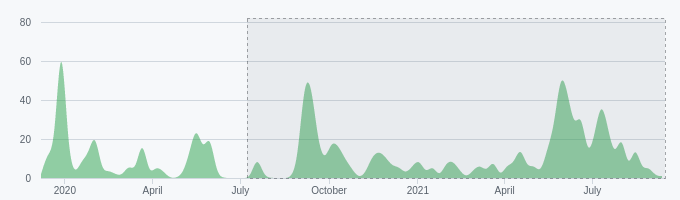
\includegraphics[width=\textwidth]{contrib.png}
  \end{block}

  \note{
    So we got lots of great new functionality, and in large part that's thanks to an influx of new contributors to the stdlib project.
    Not only has the number of modules doubles but so has the number of people who've committed changes to stdlib.
    Included in that are two Google Summer of Code students Aman Godara and Chetan Karwa, who we will hear from shortly.
    What that figure doesn't include is contributions made in the form of Issues and reviews of Pull Requests.
    It's really great to see over 100 new Issues opened in the past year, since this not only includes bug reports but also discussion of workflow improvments and proposals for new features.
    And looking at the timeline of commits since last year's FortranCon, we see a nice sustained development with big rushes of new development at the end of last summer and throughout this summer.
  }
\end{frame}


\begin{frame}
  \frametitle{stdlib is now easier to install}

  \begin{itemize}
  \item Dependencies
    \begin{itemize}
    \item Fortran compiler (supporting at least F2008)
    \item CMake (or just make)
    \item fypp preprocessor (python script)
    \end{itemize}
  \item Install each separately or use conda package manager
  \item Exports both CMake package files \& pkg-config files
  \item Support for fpm-based workflow is in progress
  \end{itemize}

  \note{
    Besides implementing and discussing new features, the other way in which stdlib has improve a lot this past year is in infrastructure.
    In particular, it's now quite straightforward to work with stdlib, whether as a developer or a user.
    So the has three dependencies: a reasonably modern Fortran compiler, a reasonably recent version of CMake (or just make if you prefer), and the fypp preprocessor, which is used mainly as a templating engine for writing generic procedures.
    These are individually not hard to install on most systems, but one might be worried about having conflicting versions of Fortran compilers or CMake on one system.
    So to address that concern and also to just serve as a very simple way to get started, there's now a conda package that will automatically install the prerequisites for stdlib.
    So then once you get the stdlib source code from Github, you can build stdlib and run its test suite with either make or CMake.
    Then when you isntall stdlib, you get not only a static or shared library but also a pkg-config file and a CMake package file, which makes it very simply to use stdlib in your own projects.
    The ideal situation of course is to distribute stdlib as an fpm package, and while that's still a work in progres, there's been good progress on the fpm side of things.
  }
\end{frame}


\begin{frame}
  \frametitle{Cross-platform support monitored with GitHub's CI workflow}

  \begin{block}{Platforms tested on every pull request}
    \begin{tabular}{llll}
      GNU & 9,10,11 & Ubuntu 20.04 & x86\_64 \\
      GNU & 9,10,11 & macOS 10.15  & x86\_64 \\
      GNU (MSYS) & 10 & Windows Server 2019 & x86\_64 \\
      GNU (MinGW) & 10 & Windows Server 2019 & x86\_64, i686 \\
      Intel classic & 2021.1 & Ubuntu 20.04 & x86\_64 \\
      Intel classic & 2021.1 & macOS 10.15 & x86\_64 
    \end{tabular}
  \end{block}
  
  \begin{itemize}
  \item If your compiler supports F2008/F2018, stdlib should compile
  \item Some require minor workarounds (NAG, some older GNU versions)
  \end{itemize}

  \note{
    The stdlib project is also leveraging Github's continuous integration workflows to check cross-platform support.
    Currently, on every pull request, the CI builds stdlib and runs its test suite on seven different platforms meaning different combinations of compiler, OS, and CPU architecture.
    However, just because your platform is not shown here doesn't mean stdlib won't work on your system.
    Anecdotally, I've built stdlib with several versions of ifort on a recent MacBook as well as several versions of gfortran on a 10-year-old netbook running 32-bit Linux.
  }
\end{frame}


\begin{frame}
  \frametitle{Room for improvement}
  
  \begin{itemize}
  \item Fill out numerical capabilities
    \begin{itemize}
    \item ``Simple'' functions are often not so simple (e.g., $cbrt$)
    \item Difficult to find reviewers with domain knowledge (see: Probability Distributions)
    \item What to put in stdlib versus create fpm package?
    \end{itemize}
    
  \item Improve consistency of documentation
    \begin{itemize}
    \item Lots of variability in style \& level of detail
    \item To be addressed with standardized tempates
    \end{itemize}
  \end{itemize}

  \note{
    I've used this talk mainly to highlight the cool new developments and accomplishments of the stdlib project so far, but there is certainly room for improvement.
    For one, most of the big exciting new modules in stdlib serve general programming needs.
    There are a couple reasons that numerical functionality has been slower to come in.
    One reason is that when one starts discussing the API and possible implementations, many ``simple'' functions turn out to have lots of subtle difficulties.
    My first-hand experience with this was in a discussion of a possible cube-root function, where one has to consider all kinds of floating-point edge cases that one wouldn't bother with in personal code but which is important to get right in a ``standard'' library.
    Another issue is that many numerical algorithms should be reviewed by people with particular domain knowledge to ensure that the implementation and tests make sense.
    The prime example of this right now is a handful of pull requests for statistical distributions that have been waiting for a reviewer with an appropriate background in statistics.
    When discussing new feature proposals, a recurring question is, ``should this be in stdlib or should this be an fpm package?''
    Really, this is a testament to the progress made with fpm, but the point is that this boundary is still being mapped out.
    The other area where the stdlib project is actively trying to improve things is in the documentation.
    Even though documentation is required for every new procedure or type, the style and rigor of this documentation varies quite a lot.
    The proposed solution right now is to establish a baseline template for specifications to follow.
    This will hopefully give the stdlib documentation a more uniform feel, as well as be a helpful starting point for new contributors.
  }
\end{frame}

\begin{frame}
  \frametitle{Summary}

  \begin{itemize}
  \item stdlib aims to be a de facto standard library of general-purpose and numerical facilities for Fortran
  \item Roughly doubled in size in the past year, both in terms of modules and contributors
  \item New modules include bitsets, logging, math utilities, sorting, special functions, RNG, and string handling
  \item Infrastructure and packaging improvments have made stdlib easier to install and use
  \end{itemize}
\end{frame}

\end{document}
